\section{Detector Calibration and Commissioning}
\label{sec:calibration}

\subsection{Pre-beam Calibration}

Initial checkout and calibrations of the FT detectors upon completion of the installation were performed via:
\begin{itemize}
    \item Pulser, LED, and cosmic ray runs for the FT-Cal;
    \item Pulser and cosmic ray runs for the FT-Hodo;
    \item Pulser and pedestal runs for the FT-Trk.
\end{itemize}

\subsubsection{FT-Cal Pre-beam Calibration}

Initial checkout of the calorimeter is performed via pulser and LED runs. In the pulser runs, an external clock is
used to trigger the readout of the entire FT-Cal recording the full FADC waveforms in a 400~ns window in the
absence of a physics signal to measure baselines and monitor noise, for the purpose of identifying disconnected
or malfunctioning channels. For each crystal, several parameters were studied, such as the average pedestal, the
event-by-event pedestal RMS, and the noise defined as the sample-by-sample pedestal RMS. The analysis was
performed online, connecting to the data acquisition Event Transfer (ET) ring~\cite{daq}, or from a recorded
EVIO file using the FT Java calibration suite~\cite{reconstruction}. Figure~\ref{fig:ftcal_pulserrun} shows a
view of a typical pulser run analysis. One the most useful information
obtained from this analysis is the average channel noise that is indicative of its functionality: a noise level below
the typical range is indicative of a malfunctioning preamplifier or a disconnected cable, while a noise level above the
typical range can indicate a high-voltage issue since the noise introduced by the LAAPDs is higher when the biased
voltage is not applied. 

\begin{figure}
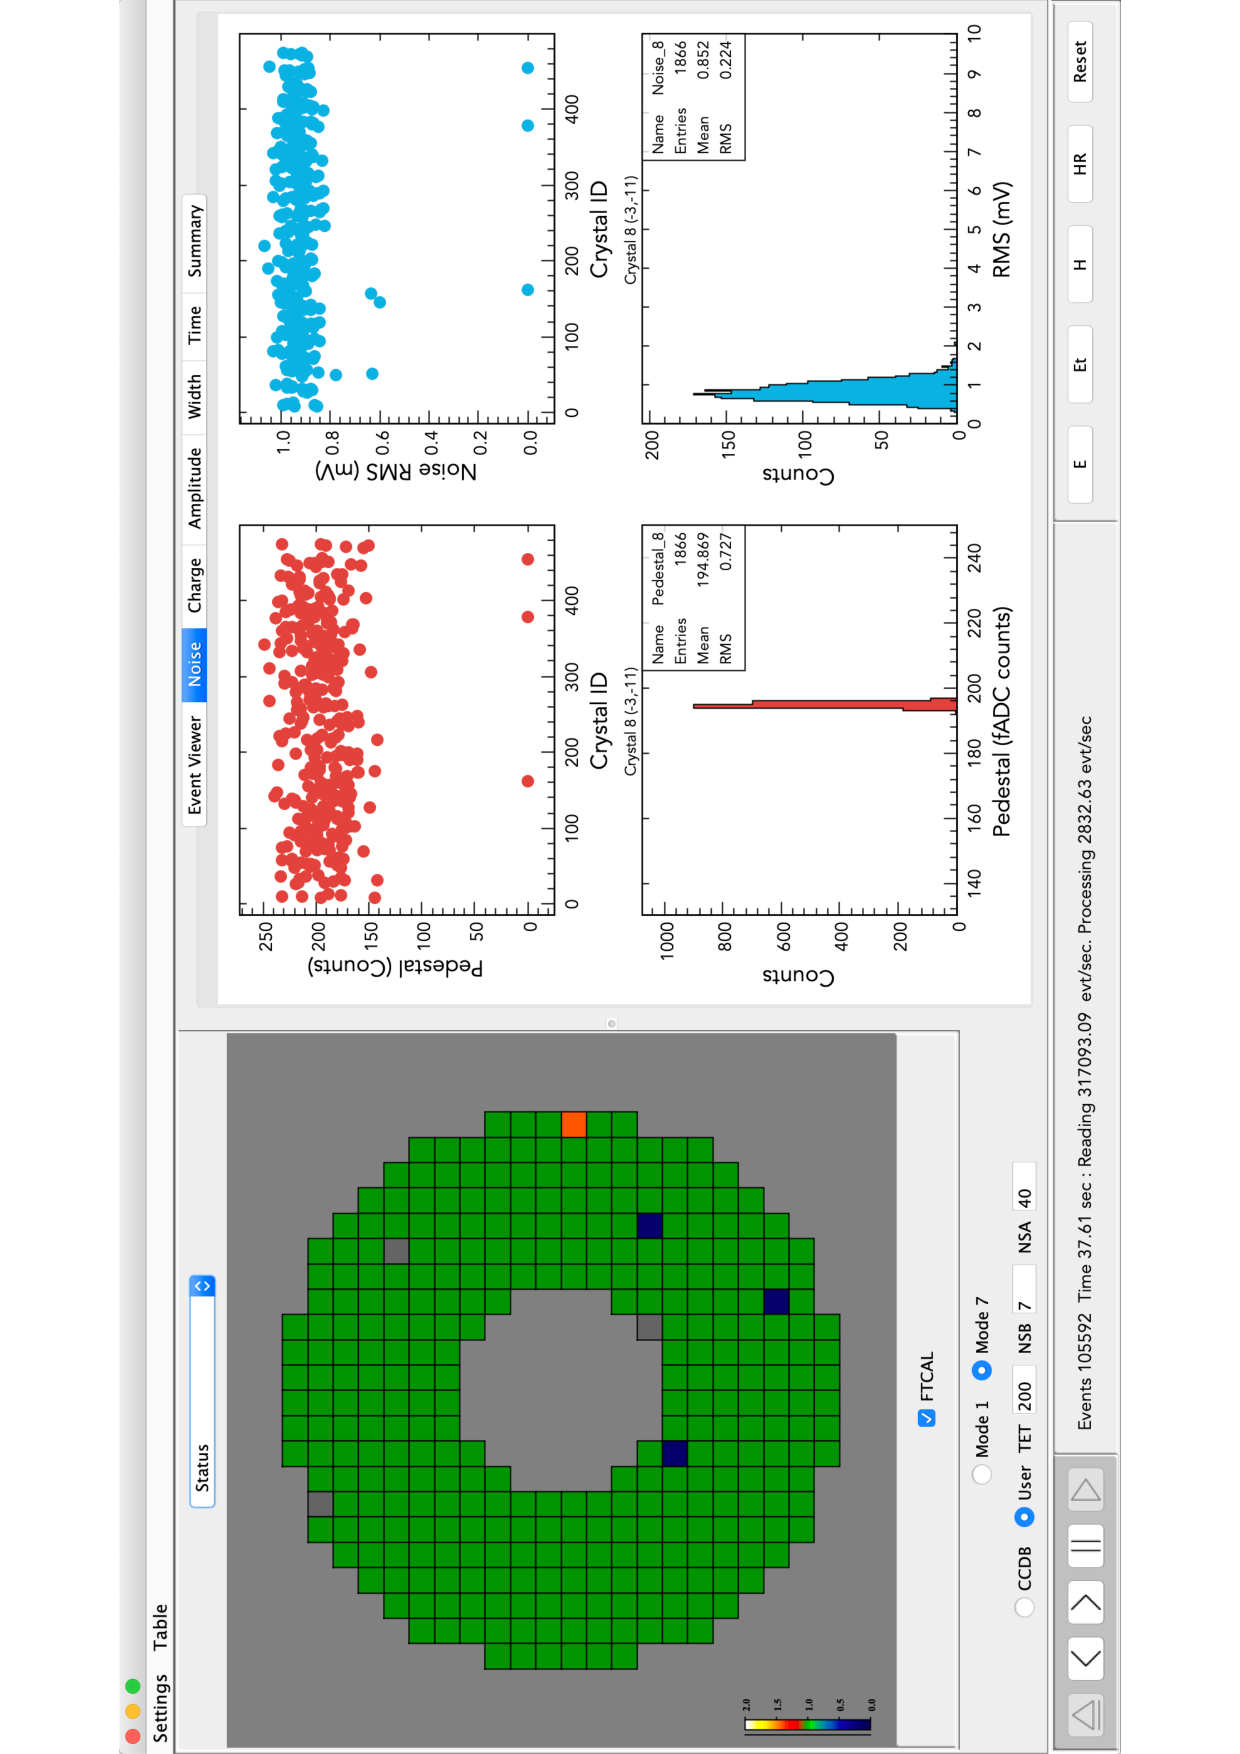
\includegraphics[height=1.0\columnwidth,angle=270]{fig/ftcal_pulserrun.pdf}
\caption{Results of the FT-Cal noise analysis from a pulser run. The left part of the calibration suite display shows a
  view of the calorimeter with a color scheme representing the status of the crystal: green corresponds to a fully
  functional element, blue to an element with noise below the typical range that is indicative of a low gain preamplifier,
  orange to an element with noise above the typical range, and gray to a crystal for which no data were recorded. The
  right part of the panel shows the average pedestal and noise as a function of the crystal number, and the event
  distribution of the pedestal and noise for the selected crystal.}
\label{fig:ftcal_pulserrun}
\end{figure}

Once the initial debugging of the system based on pulser runs is completed, a second checkout based
on LED runs is performed. In this case, the FT-Cal LMS is used to input light into each of the calorimeter crystals and the
corresponding signals are recorded to check the pulse amplitude and shape, and assess the correct functioning of
the LAAPDs, preamplifiers, and front-end electronics. Using the EPICS slow controls interface of the LMS, the LEDs
are switched on in groups of 6, one per driver, in a predefined sequence and pulsed at a rate of 62.5~Hz for a time
interval of 30~s to accumulate about 1800 waveforms per channel. The LED pulse amplitudes have been tuned to
provide a maximum amplitude at the FADC of about 1~V, which is representative of a typical signal expected for the
calorimeter. The recorded waveforms are analyzed to extract the pulse amplitude as a function of time. In fact, upon
being turned on, the LED light intensity undergoes an exponential drop until it reaches stability. This happens typically
within 6-8~s. The amplitude in the stability region is fitted to a constant to extract the average value that is recorded
and compared to reference values to detect changes in the detector response and potential failures.
Figure~\ref{fig:ftcal_ledrun} shows the results of the analysis of a typical LED run as displayed by the calibration
Graphical User Interface (GUI). In this specific case, the analysis shows a relatively uniform response to the LED light,
with typical amplitudes on the order of 1~V as defined by design, with few problematic channels that coincide with those
identified by the pulser runs of Fig.~\ref{fig:ftcal_pulserrun}. 

\begin{figure}
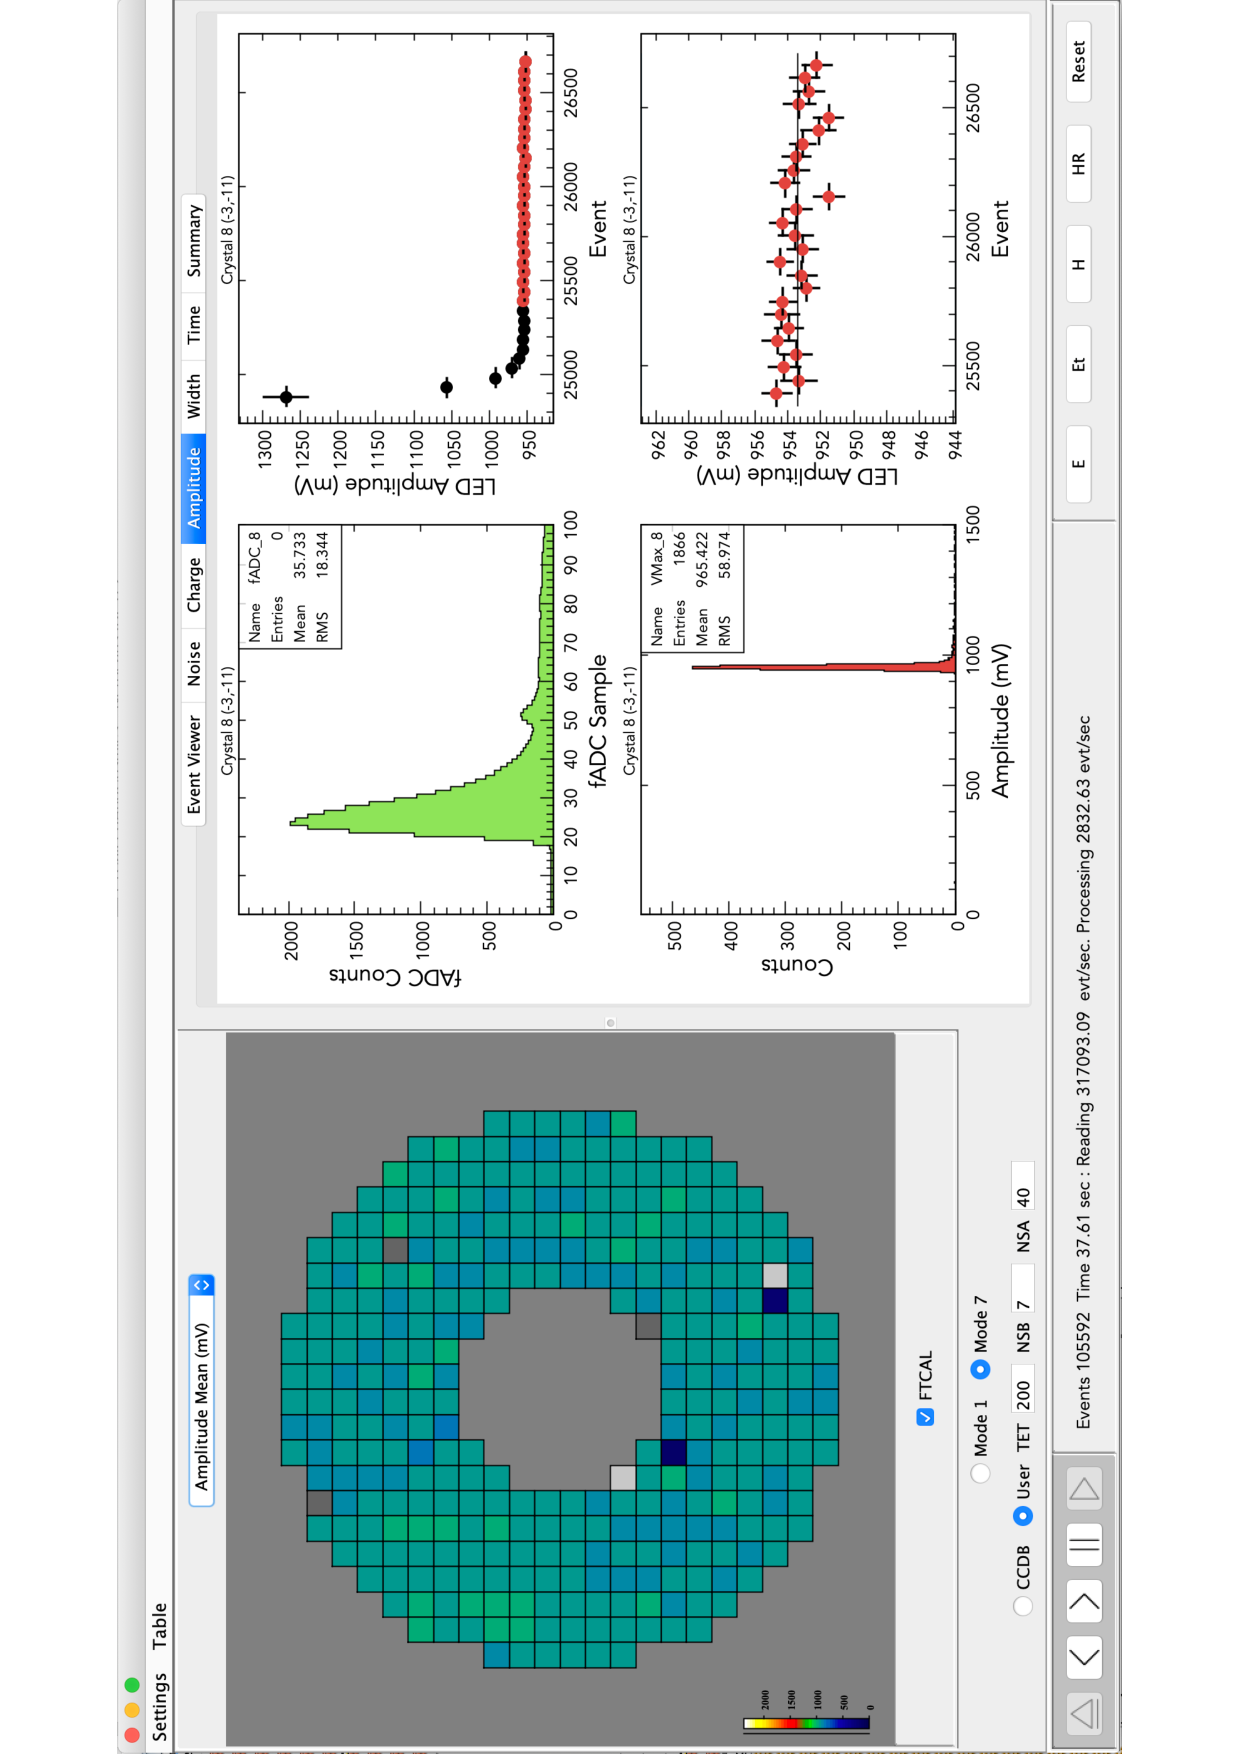
\includegraphics[height=1.0\columnwidth,angle=270]{fig/ftcal_ledrun.pdf}
\caption{Results of a typical FT-Cal LED run. The left part of the calibration suite display shows a view of the
  calorimeter with a color scheme representing the LED pulse amplitude. The right part of the panel shows for the
  selected crystal the average pulse shape (top left), the pulse amplitude as a function of the event number, i.e. of
  time (top right), the distribution of the amplitudes (bottom left), and the pulse amplitude  as a function event number
  after the LED has reached stability (bottom right). The latter is fitted to a constant to determine the pulse
  amplitude that is displayed in the detector view.}
\label{fig:ftcal_ledrun}
\end{figure}

The final calibration of the FT before in-beam testing was based on the study of the detector response to cosmic
rays. A special FPGA-based trigger was developed by the JLab Fast Electronics Group to select events where a
cosmic ray crosses the calorimeter primarily in the vertical direction, i.e. crossing the crystals along the short side.
This is achieved by requiring a minimum number of signals above threshold in the crystals that are in a ``column'' of
the calorimeter assembly, a technique that exploits the functionalities of the JLab FADCs and trigger electronics
~\cite{daq,trigger}. For these events, the waveforms for all crystals in the calorimeter were recorded and analyzed
offline using the FT-Cal calibration suite. Details of the analysis procedure are reported in
Refs.~\cite{cosmics1,cosmics2}; here we summarize only the main steps and results. For each crystal, events where
at least $N_{min}$ crystals with signal above threshold are found in a vertical range of $N_{range}$ crystals above or
below the chosen one. After optimization, the values of $N_{min}$ and $N_{range}$ were fixed to 4 and 5, respectively.
For these events, the crystal waveform was integrated in a fixed range and pedestal subtracted to extract the
charge. The integration range was optimized empirically to maximize the signal-to-noise ratio. The charge distribution
for all selected events in the given crystal was then fitted with a Landau summed with an exponential function,
representing the minimum-ionizing particle deposition and background, respectively. The mean of the Landau function,
compared with the expected average energy deposition determined from Geant4 Monte Carlo simulations to be
15.3~MeV, was then used to evaluate the charge-to-energy conversion factor for each crystal. 

\begin{figure}
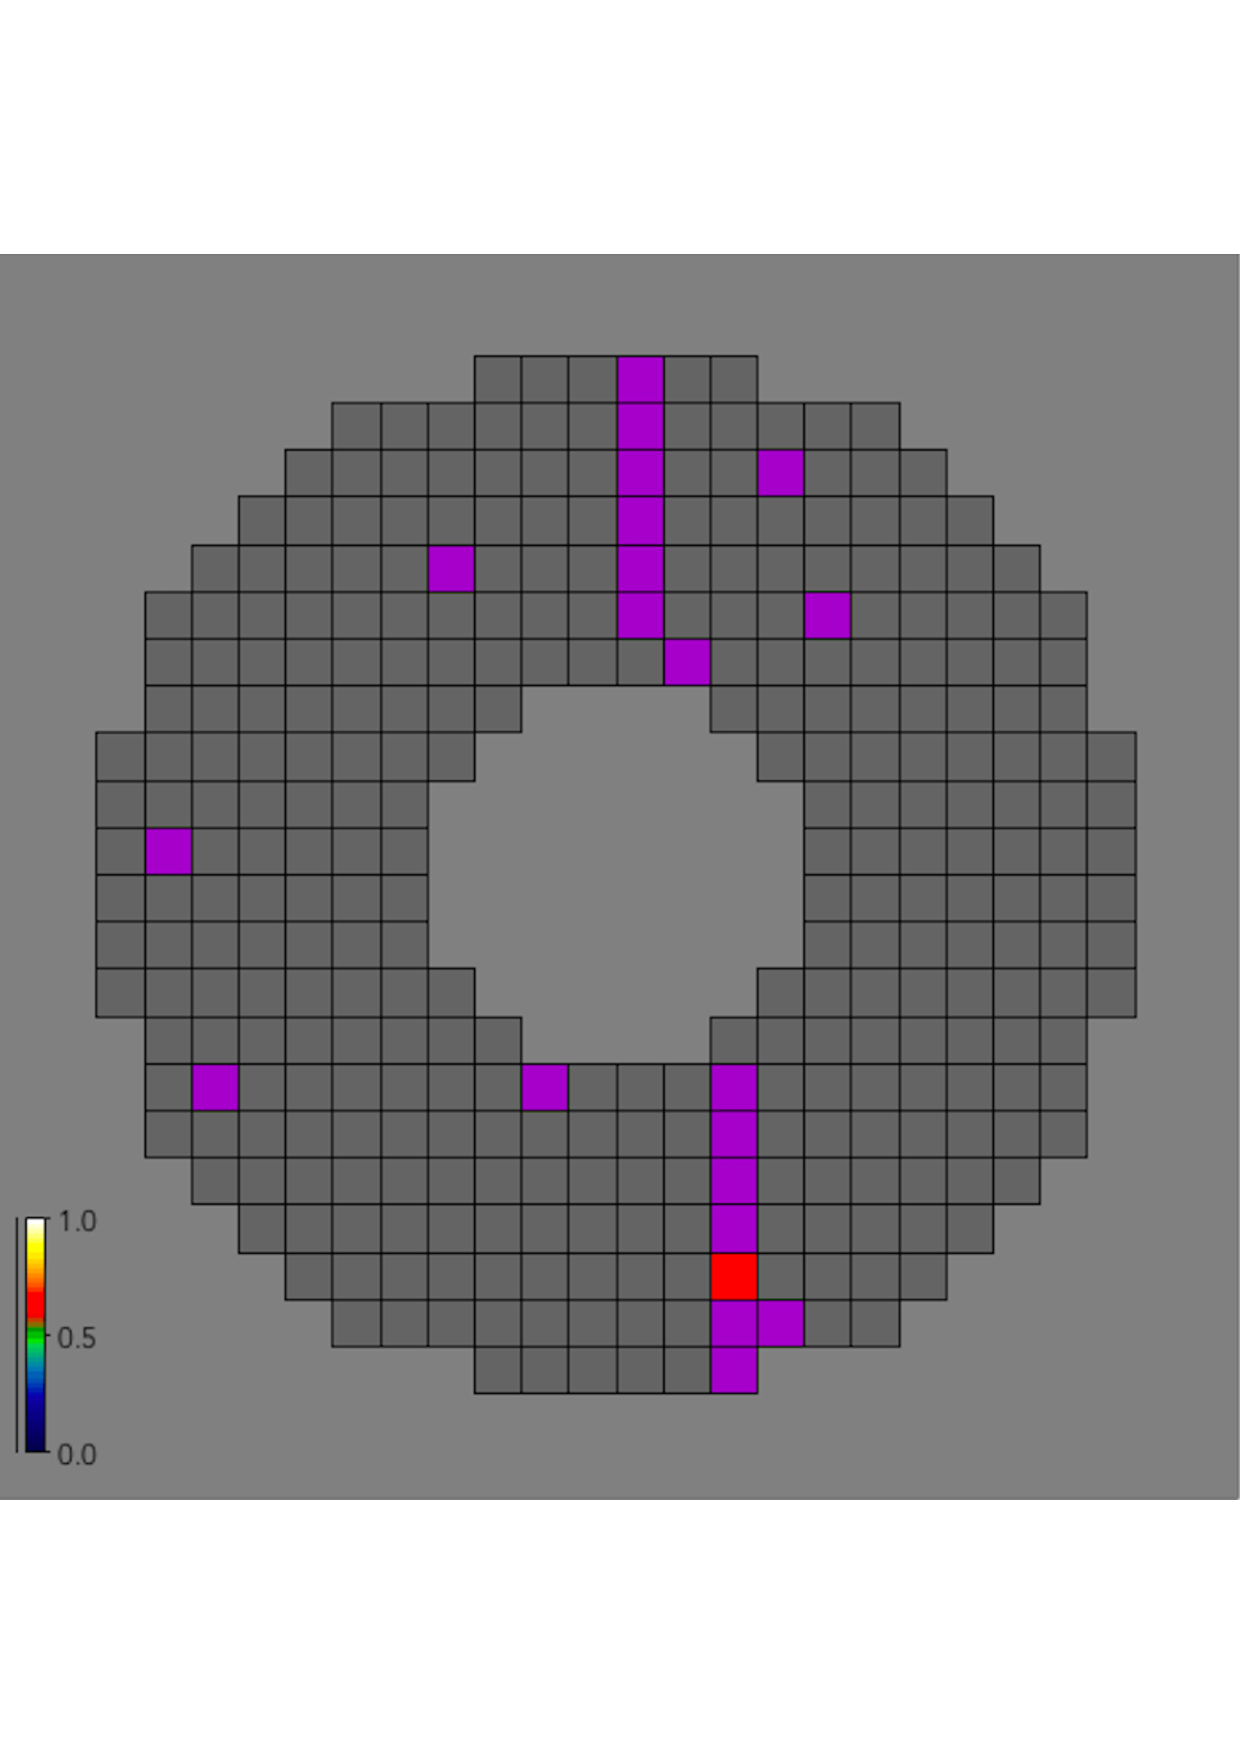
\includegraphics[height=0.58\columnwidth]{fig/ftcal_cosmicview.pdf}
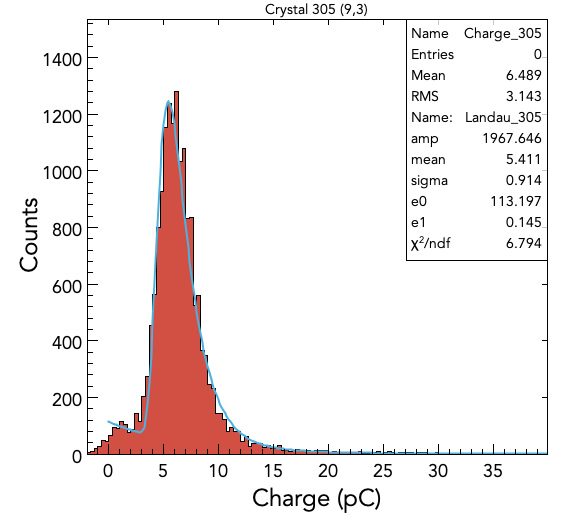
\includegraphics[height=0.5\columnwidth]{fig/ftcal_cosmiccharge.png}
\caption{Left: example of a cosmic ray crossing the calorimeter vertically as displayed by the calibrations suite.
  Right: example of the measured charge distribution measured from the selected events for a calorimeter crystal;
  the blue line shows the results of the Landau plus exponential fit; the mean of the Landau function is used to
  estimate the charge-to-energy conversion factors.}
\label{fig:ftcal_cosmic}
\end{figure}

Figure~\ref{fig:ftcal_cosmic} shows an example of a cosmic ray event as displayed by the calibration suite and an
example of the charge distribution for a selected crystal obtained by integrating over the selected events. The
typical values of the Landau peak were found to be in the range of 4-7~pC at the calorimeter operating temperature
of $0^\circ$C and the corresponding conversion factors in the range of 2.2-3.8~MeV/pC. These values were used as
the calibration constants for the initial reconstruction of beam data, although it was found that these constants
usually led to an overestimate of 20\% of the actual energy deposited in the energy range of interest for the
calorimeter of 0.5-4.5~GeV. While this discrepancy is significant, it is not unexpected given the uncertainties in
extracting the cosmic ray signal from the background and the 
large difference in the two calibration points, since cosmic rays deposit an energy in the range of tens MeV while the energy range  for beam-induced signals is two orders of magnitude larger.

\subsubsection{FT-Hodo Pre-beam Calibration}

Similarly to the calorimeter, initial checkout of the hodoscope was performed via pulser runs to check the functionality
of each electronic channel and evaluate the SiPM gains by measuring the single photoelectron (SPE) signal. An external
clock was used to trigger the data acquisition recording the waveform of all the 232 channels in a 400~ns windows.
The waveforms could be analyzed online by connecting the calibration suite to the data acquisition ET ring~\cite{daq}
or offline reading from file. The parameters that were monitored are the pedestal values, the pedestal RMS, and the
electronic noise. The extracted SPE values were compared to the typical ones to identify problematic channels and
disconnected cables. For each channel, the waveforms that exceeded a minimum threshold above the baselines were
analyzed to extract the SPE signal. For this purpose, the waveforms were integrated in a fixed time range and pedestal
subtracted. The distribution of the extracted charge for a selected channel is shown in Fig.~\ref{fig:fthodo_spe}, where the top and bottom plots are for the same tile in the two detector layers and the left and right plots show the results obtained using the waveform maximum and integral, respectively.
Clear peaks corresponding to one, two, and three photoelectrons are visible; the difference between two peaks was used
to determine the gain of the channel, resulting in typical values on the order of 20~pC. The consistency of the results obtained using the pulse maximum and integral confirms the reliability of the waveform analysis.

\begin{figure}
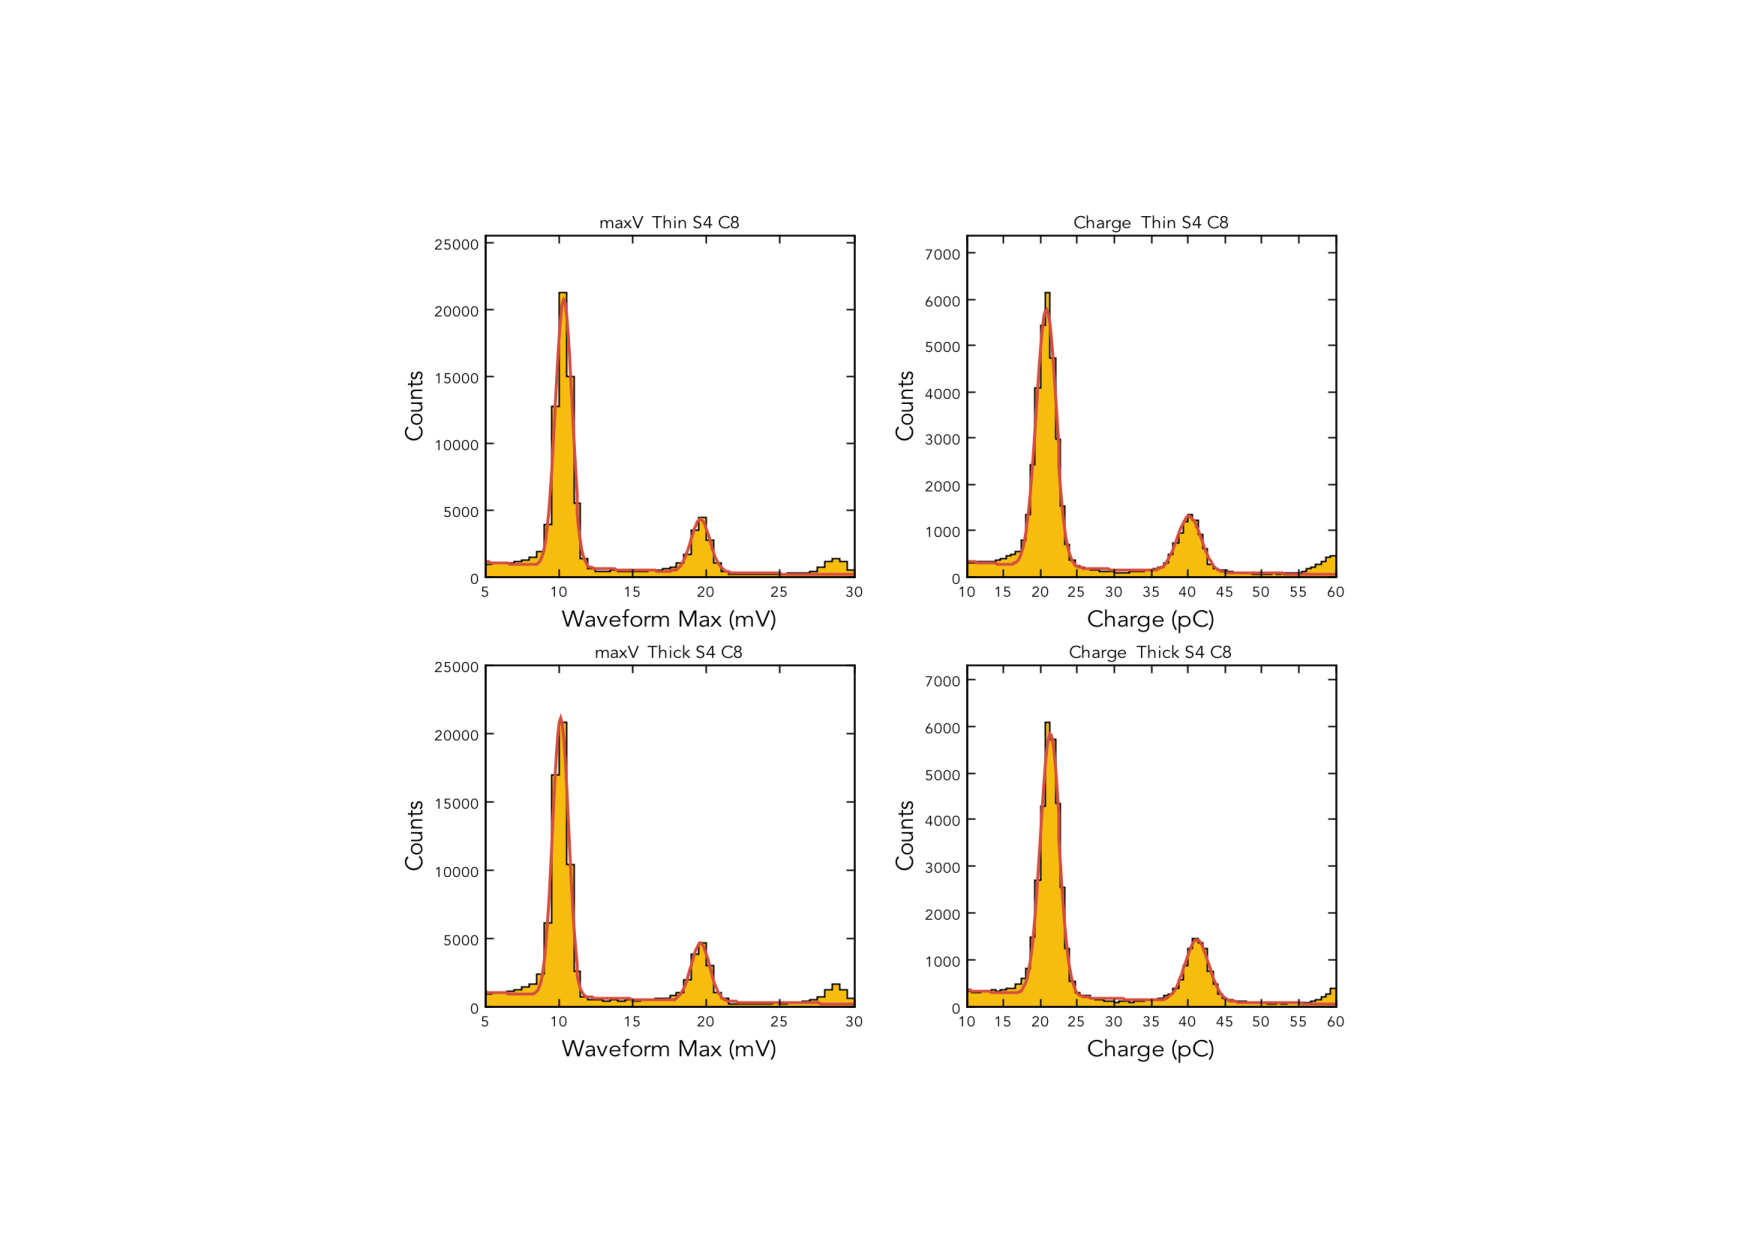
\includegraphics[width=1.0\columnwidth]{fig/fthodo_spe_2.pdf}
\caption{SPE signal from the FT-Hodo SiPMs reading signals from the thin (top) and thick (bottom) tiles, in mV
  (left) and pC (right) determined using the waveform maximum and integral, respectively.}
\label{fig:fthodo_spe}
\end{figure}

Further checkout of the detector is performed via cosmic ray data taking. The same FPGA-based trigger developed
for the calorimeter is used to trigger the data acquisition system on events in which multiple tiles of the hodoscope
have a signal above threshold. For such events, all hodoscope channel waveforms are recorded and analyzed offline.
The signal charge is extracted integrating the waveform in a fixed time window and subtracting the pedestals. The
resulting charge distributions are inspected to ensure a sizable signal for all tiles. In this case no attempt is made to
extract the charge-to-energy conversion factor from these distributions because of the unfavorable orientation of
the hodoscope in the installation position for the measurement of cosmic rays that can cross the scintillation tiles with
a very large angular and energy deposition spread.

\subsubsection{FT-Trk Pre-beam Calibration}

First calibration and test of the detectors was performed using the cosmic-ray test bench available at
CEA-Saclay~\cite{mm}. The goal of these tests was to optimize the operating conditions of the detectors and to
compute their 2D efficiency maps using cosmic muons prior to shipment to JLab. Figure~\ref{fig:ftt_cosmic} shows
the results for two of the four detector layers, indicating a good uniformity of the response over the full active area.

\begin{figure}[htb]
 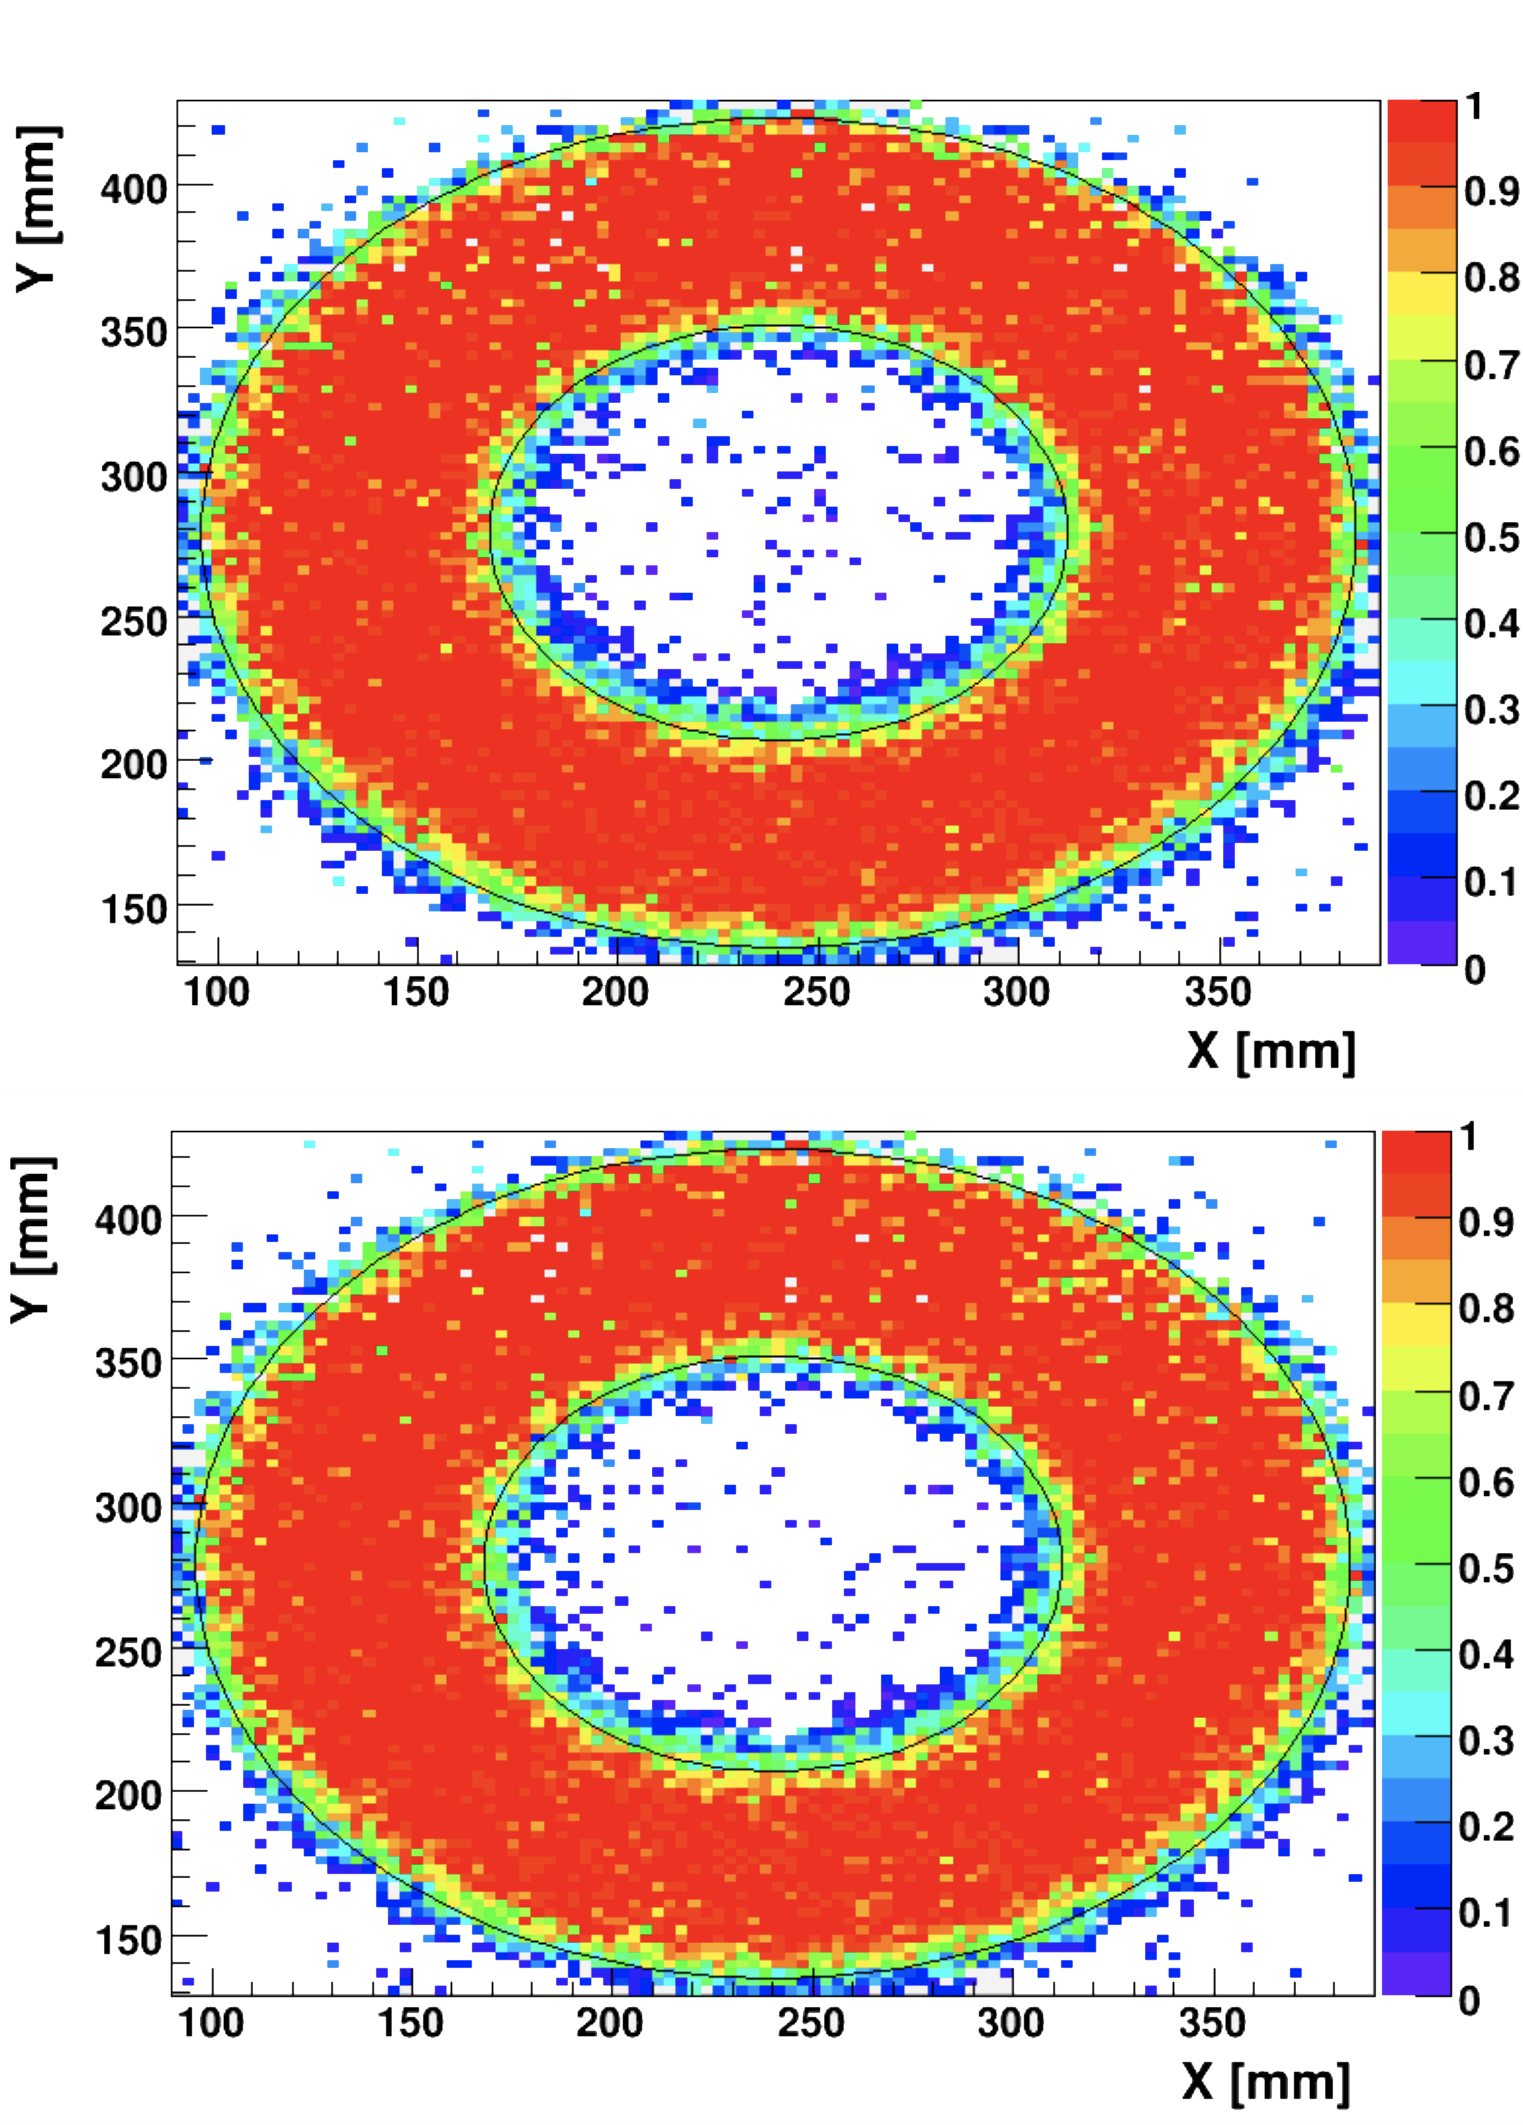
\includegraphics[width=0.9\columnwidth,keepaspectratio]{fig/fttrk_cosmic.png}
 \caption{2D efficiency map for the two layers of one of the FT tracker detectors as measured in the cosmic-ray
   setup at CEA-Saclay. The black circles indicate the limits of the detector active area.}
 \label{fig:ftt_cosmic}
\end{figure}

After installation, the initial checkout of the FT-Trk and, in particular, of the front-end electronics, was performed
by means of pedestal and pulser runs. Since these procedures are standard for the CLAS12 Micromegas detectors,
we refer to Ref.~\cite{mm} for further details.

\subsection{In-beam Calibration and Commissioning}

While pre-beam calibrations were essential to ensure all detector components were fully operational, the final
calibrations to extract the parameters needed for the FT reconstruction are based on analysis of beam data.
Here we report specifically on the procedures developed for the calibration of the calorimeter and hodoscope,
since no specific calibrations are needed for the tracker.

For both the hodoscope and calorimeter, energy and time calibrations can be obtained from the analysis of data
recorded with the CLAS12 production triggers and do not require dedicated data taking. A dedicated run is
typically employed, however, for matching the gains from all FT-Hodo SiPMs~\footnote{Having a matched gain
from all FT-Hodo SiPMs allows for a common trigger readout threshold for all channels.}. In this dedicated run,
average minimum-ionizing particle signals were obtained for a set of different HV settings (see
Fig.~\ref{fig:fthodo_gainmatch}), determining two constants from which gain matching is established.

\begin{figure}
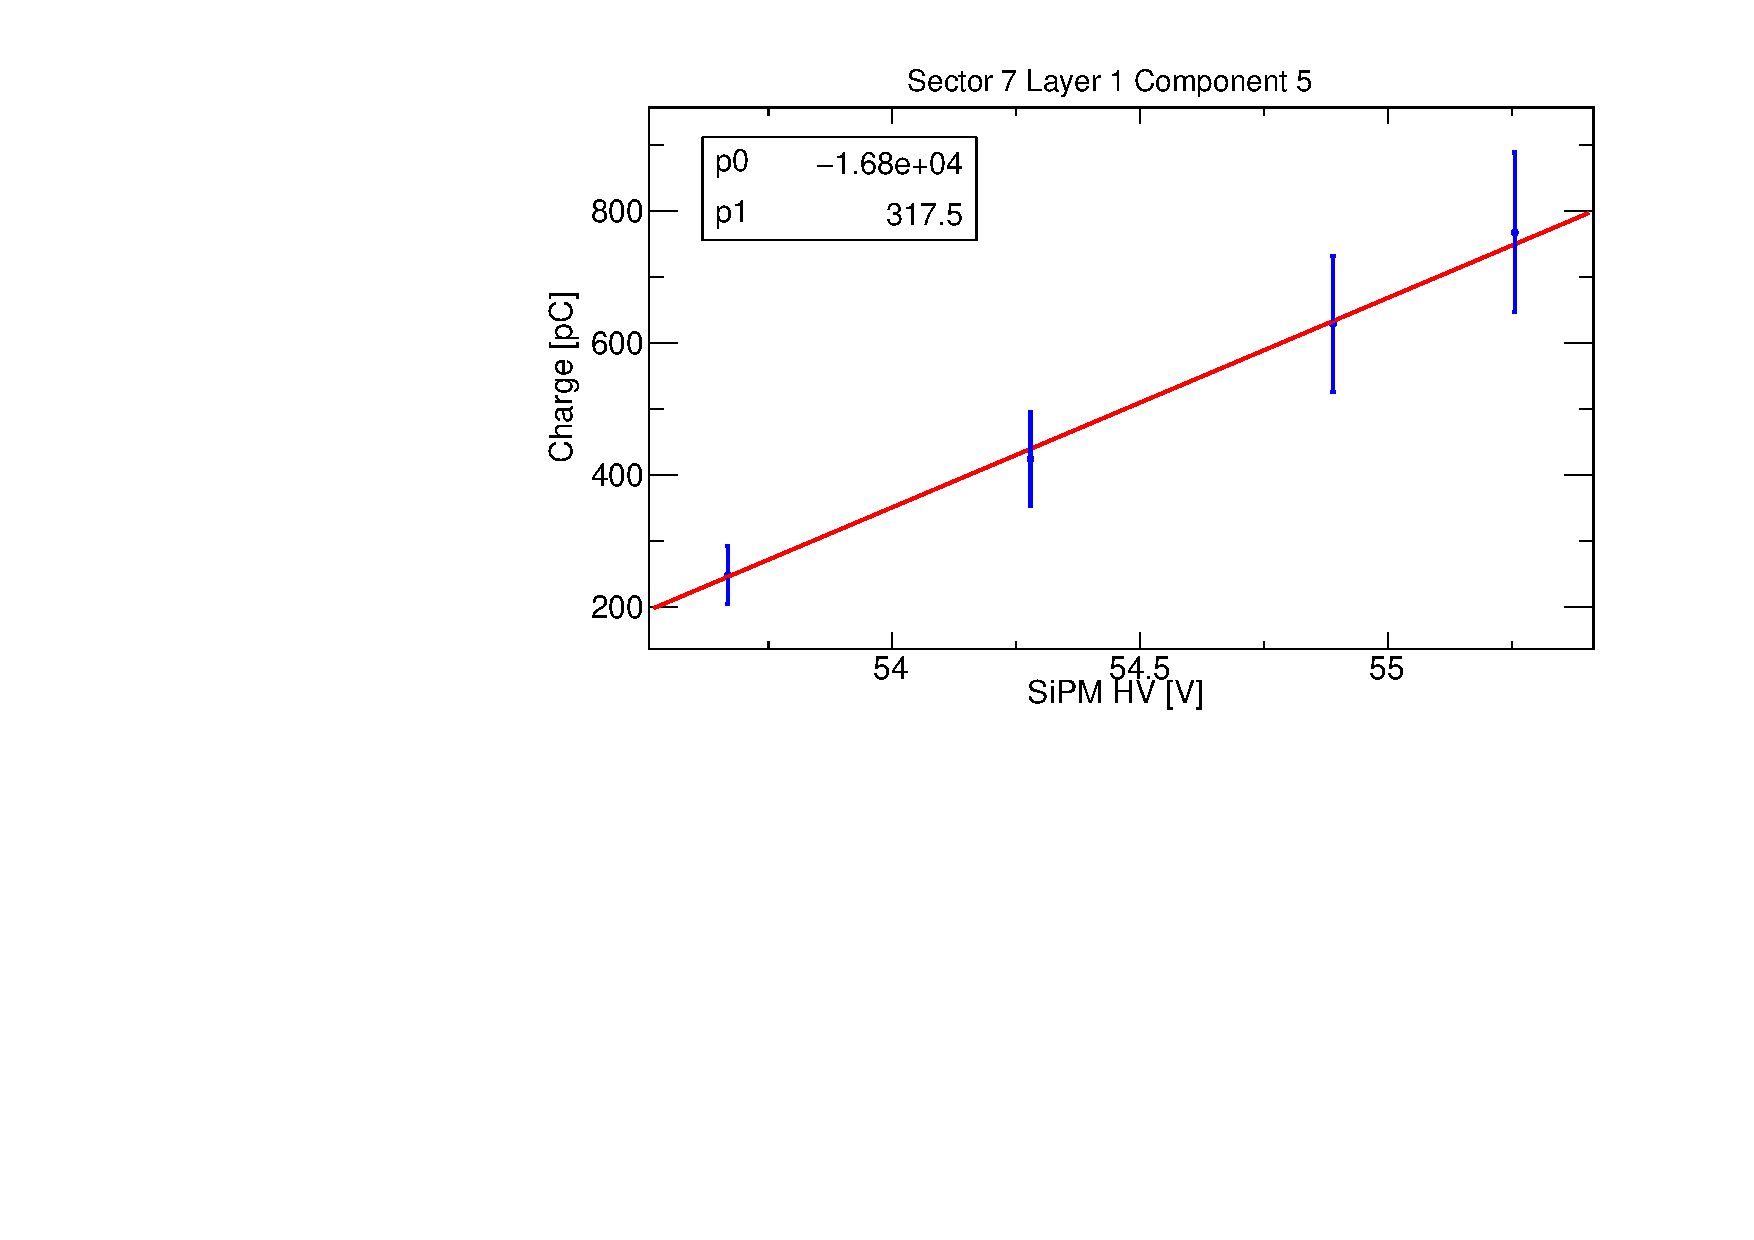
\includegraphics[width=1.0\columnwidth]{fig/fthodo_gainmatch.pdf}
\caption{Dependence of the MIPS mean position on the SIPM bias voltage for a single hodoscope tile. The dependence is fitted to a linear function that is used to select the operating voltage that would give an average MIP signal close to the chosen value.}
\label{fig:fthodo_gainmatch}
\end{figure}

The energy calibration for the FT-Cal is achieved by analyzing electron elastic scattering events or by reconstructing
the $\pi^0\to\gamma\gamma$ decay where both photons are detected in the calorimeter. 

\begin{figure}
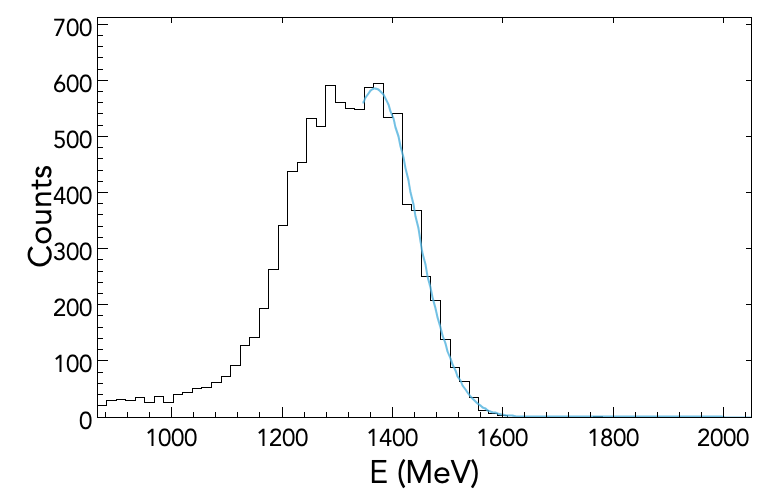
\includegraphics[width=0.9\columnwidth]{fig/ftcal_elastic_seed.png}
\caption{Example of the seed energy distribution and the cluster energy distribution for a selected crystal for
  elastic events at 2.2~GeV beam energy.}
\label{fig:ftcal_elasticcal}
\end{figure}

Elastic scattering calibration was found to be particularly effective at low beam energy and was performed using
2.2~GeV beam data recorded during the CLAS12 engineering run. Events with only one cluster in the FT-Cal were
selected and, based on the existing cosmic ray calibrations, the energy of the crystal with the largest signal, i.e. the
{\it seed}, was extracted. For each crystal, these events were accumulated requesting the seed energy to be larger
than 55\% of the total cluster energy. The right edge of the distribution of the seed energy was fitted with a
Gaussian function to extract the peak position. The mean value of the Gaussian function was compared to what
expected based on Geant4 Monte Carlo simulations to extract a correction to the charge-to-energy conversion factor
used in the cluster reconstruction. Figure~\ref{fig:ftcal_elasticcal} shows an example of the seed energy distribution
and the cluster energy distribution for a selected crystal. Using these constants, an energy resolution of 3.3\% at
2.2~GeV beam energy was determined by fitting the reconstructed elastic peak (see Fig.~\ref{fig:ftcal_elasticres}).
With the same calibration constants, the $\pi^0\to\gamma\gamma$ decay was reconstructed at 10.6~GeV beam
energy selecting events with both photons detected in the FT-Cal, finding the width of the $\pi^0$ peak to be
$\sim$4.4~MeV, i.e. $\sim 3.2\%$.

\begin{figure}[t]
\centering
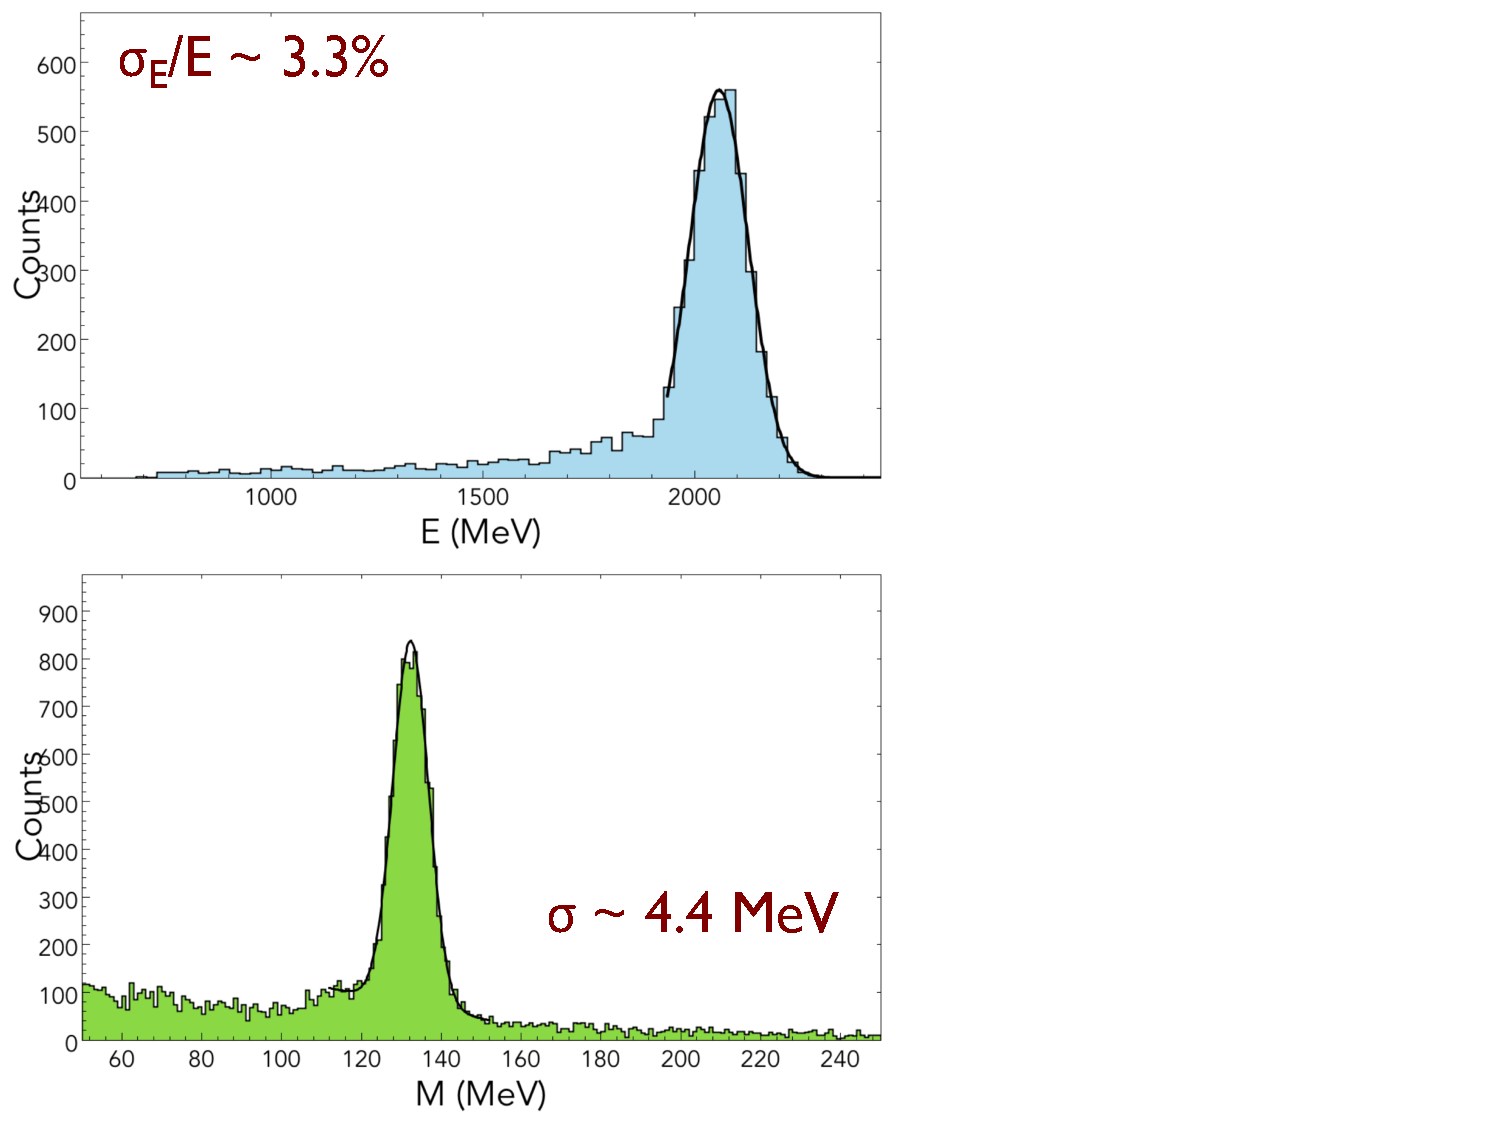
\includegraphics[height=1.0\columnwidth]{fig/ftcal_elasticres.pdf}
\caption{Top: electron energy spectrum reconstructed at 2.2~GeV beam energy in the FT-Cal; the peak corresponds
  to elastic scattering; after calibrations based on elastic events, an overall energy resolution of 3.3\% at 2.2~GeV is
  found. Bottom: $\pi^0\to\gamma\gamma$ invariant mass spectrum reconstructed at 10.6 GeV beam energy using the
  elastic scattering energy calibrations: the width of the $\pi^0$ peak determined via a Gaussian fit was found to be
  $\sim$4.4~MeV.}
\label{fig:ftcal_elasticres}
\end{figure}

Since the effectiveness of the elastic calibration is limited to beam energies of the order of a few GeV because of
the rapid decrease of the corresponding cross section at higher energies, an alternative approach was developed to
perform the energy calibration of the FT-Cal based on $\pi^0\to\gamma\gamma$ decays. Events where both
photons are detected in the calorimeter were selected and filtered applying the following cuts:
\begin{itemize}
    \item the energy of both clusters, as reconstructed based on existing calibrations, is larger than 500~MeV,
    \item the size of both clusters, i.e. the number of crystals involved, is larger than 3,
    \item the opening angle between the two clusters is larger than $2^\circ$.
\end{itemize}

The last cuts are useful to reduce background resulting from split clusters, i.e. events in which a secondary particle originating from the electromagnetic shower create a second cluster at close distance from the primary one.  For each crystal, events in which the
crystal is the seed of one of the two clusters are accumulated and the ratio between the measured cluster energy
for the given crystal and the energy calculated from the nominal $\pi^0$ mass and the other cluster energy is
computed. The distribution of such ratios is fitted with a Gaussian function to derive a correction factor for the
charge-to-energy calibration constant of the selected crystal. The procedure is applied iteratively until the $\pi^0$
mass spectrum for all crystal is within 0.5~MeV of the nominal value. Figure~\ref{fig:ftcal_pi0} shows an example of
the ratio distribution and of the $\pi^0$ mass spectrum for a selected crystal before and after (blue histogram)
the calibration procedure. The advantage of this procedure is that it does not strongly depends on the beam energy
and exploits the full energy spectrum of the clusters providing a check of the linearity. The left panel of
Fig.~\ref{fig:ftcal_pi0res} shows the  correlation between the measured and computed cluster energies after
calibration: the energy range, which is covered with good statistics, is from 0.5 to 5~GeV with a perfect overlap with
the energy range of interest for the FT. The resolution that is achieved with this calibration algorithm is of the order
of 4-5~MeV integrated over the entire calorimeter as  shown by the right panel of Fig.~\ref{fig:ftcal_pi0res}.

\begin{figure}
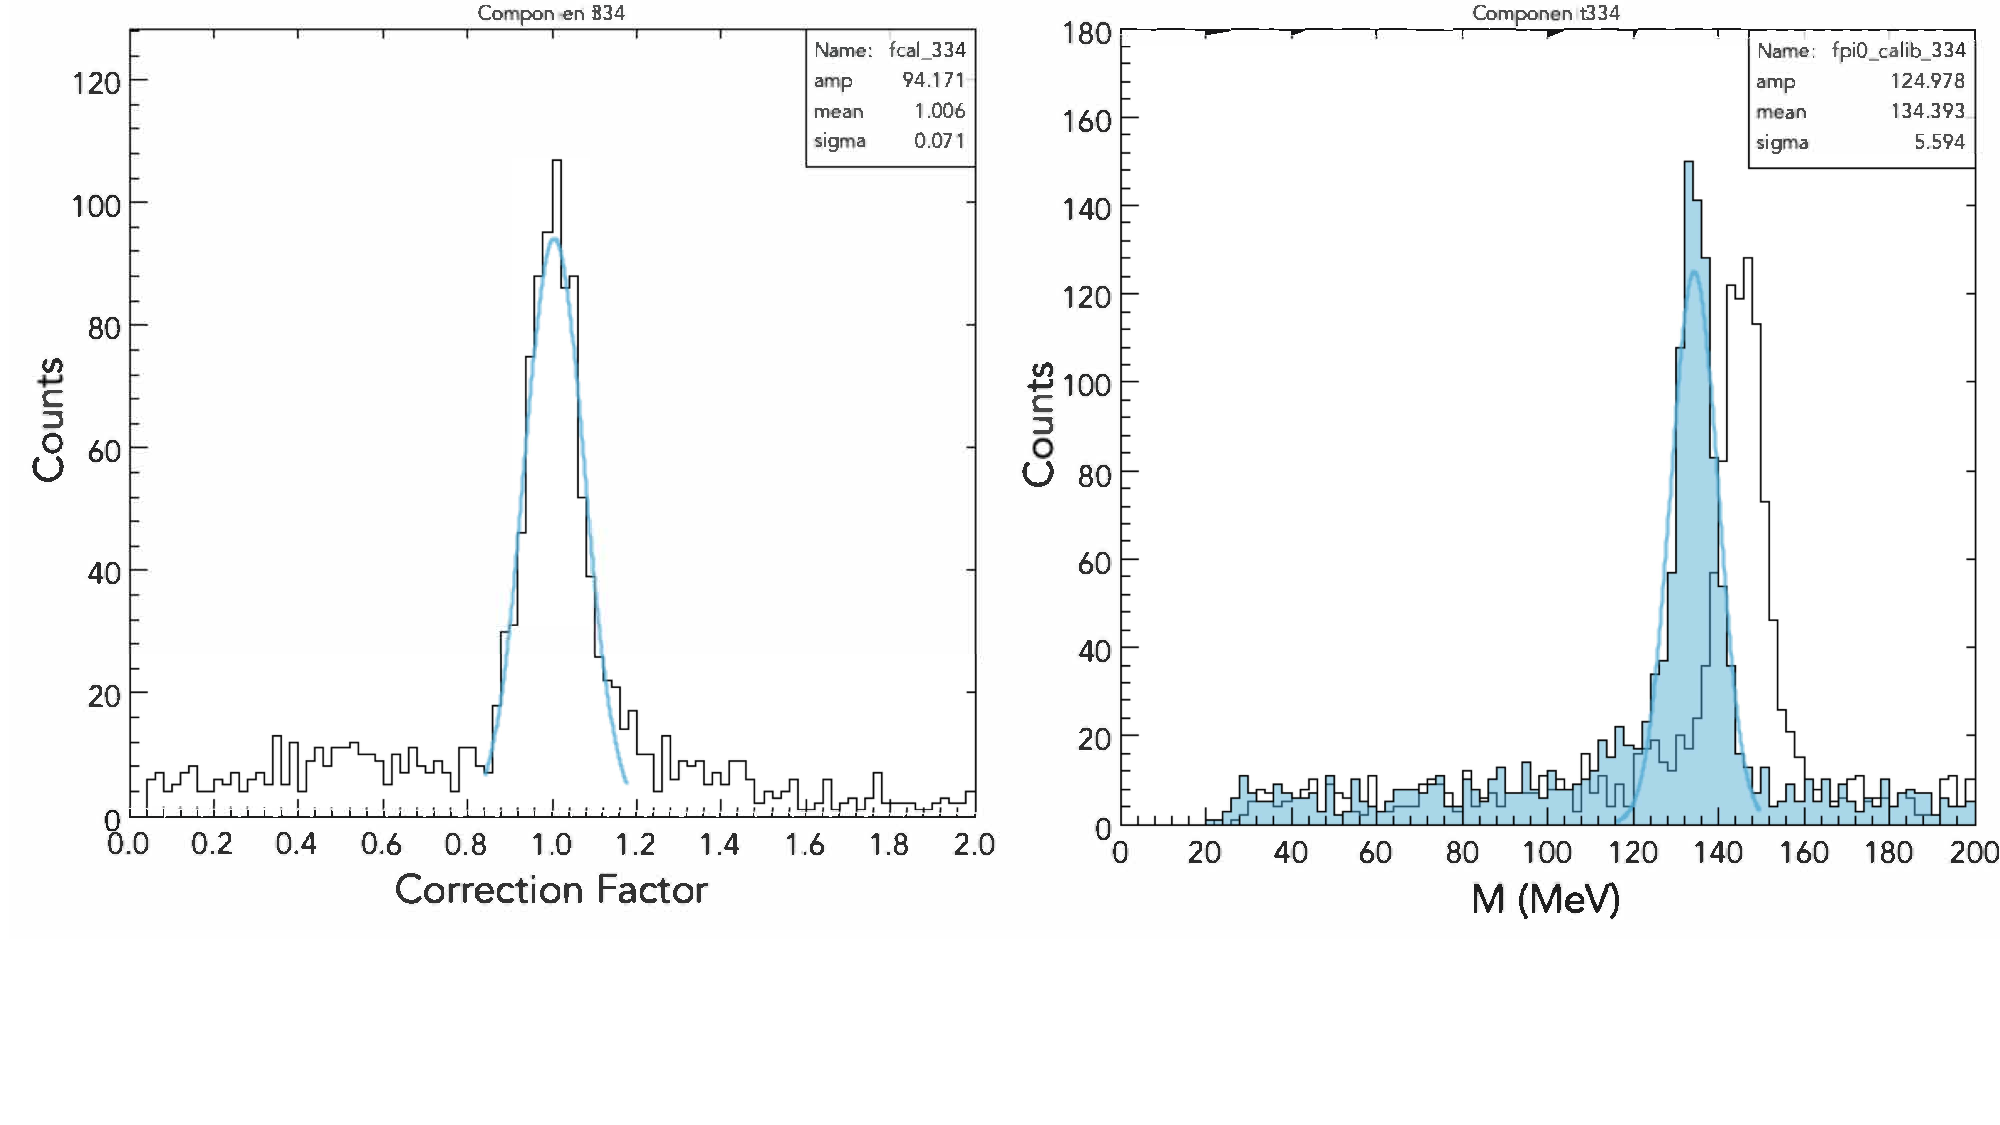
\includegraphics[height=0.46\columnwidth]{fig/ftcal_pi0.pdf}
\caption{Left: calibration correction factor for a selected crystal computed as the ratio between the measured
  energy of clusters where the crystal is the seed and the energy calculated from the nominal $\pi^0$ mass and the
  other cluster energy. Right: $\pi^0$ mass spectrum for the same crystal before and after the calibration procedure.}
\label{fig:ftcal_pi0}
\end{figure}

\begin{figure}
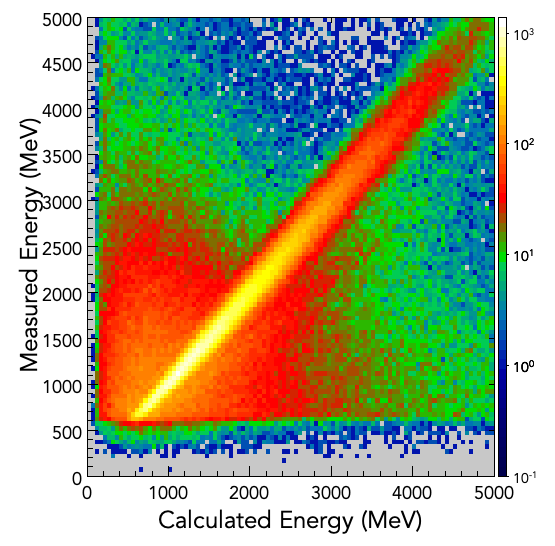
\includegraphics[height=0.48\columnwidth]{fig/ftcal_pi0linearity.png}
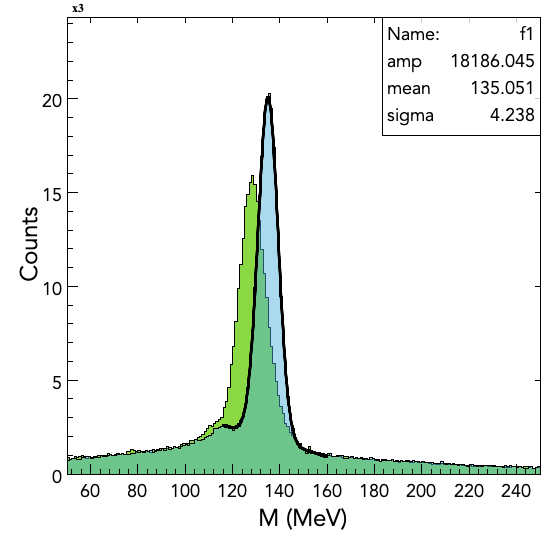
\includegraphics[height=0.48\columnwidth]{fig/ftcal_pi0resolution.png}
\caption{Left: correlation between the measured cluster energy and the energy computed from the nominal $\pi^0$
  mass; the range covered is well match to the FT energy range of interest. Right: $\pi^0$ mass spectrum before
  (green) and after (blue) the calibration; the achieved resolution is $\sim$4.2~MeV.}
\label{fig:ftcal_pi0res}
\end{figure}

{\color{green} The energy calibration of the FT-Hodo is performed by studying the energy deposition of minimum ionizing particles
(MIPs), since these are the typical signals expected charged particles impinging on the detector. Figure~\ref{fig:fthodo_mips} shows the charge from MIP signals in the thin and thick tiles. For the FT-Hodo,
charged particle signals are selected by requiring the geometrical matching of tiles in the two layers. No other requirement or matching with other detectors is requested to minimize the dependency on other systems calibration. The
distributions are fit with a Landau plus an exponential function to determine the average MIP charge. The
charge-to-energy conversion factors are determined by comparing the resulting values to the ones estimated from
Geant4 Monte Carlo simulations. The constant values were found to be very stable with time, requiring the calibration to be performed only at the beginning of a new data taking period or after a change of the detector operating conditions as for example a change of the HV settings.}

\begin{figure}
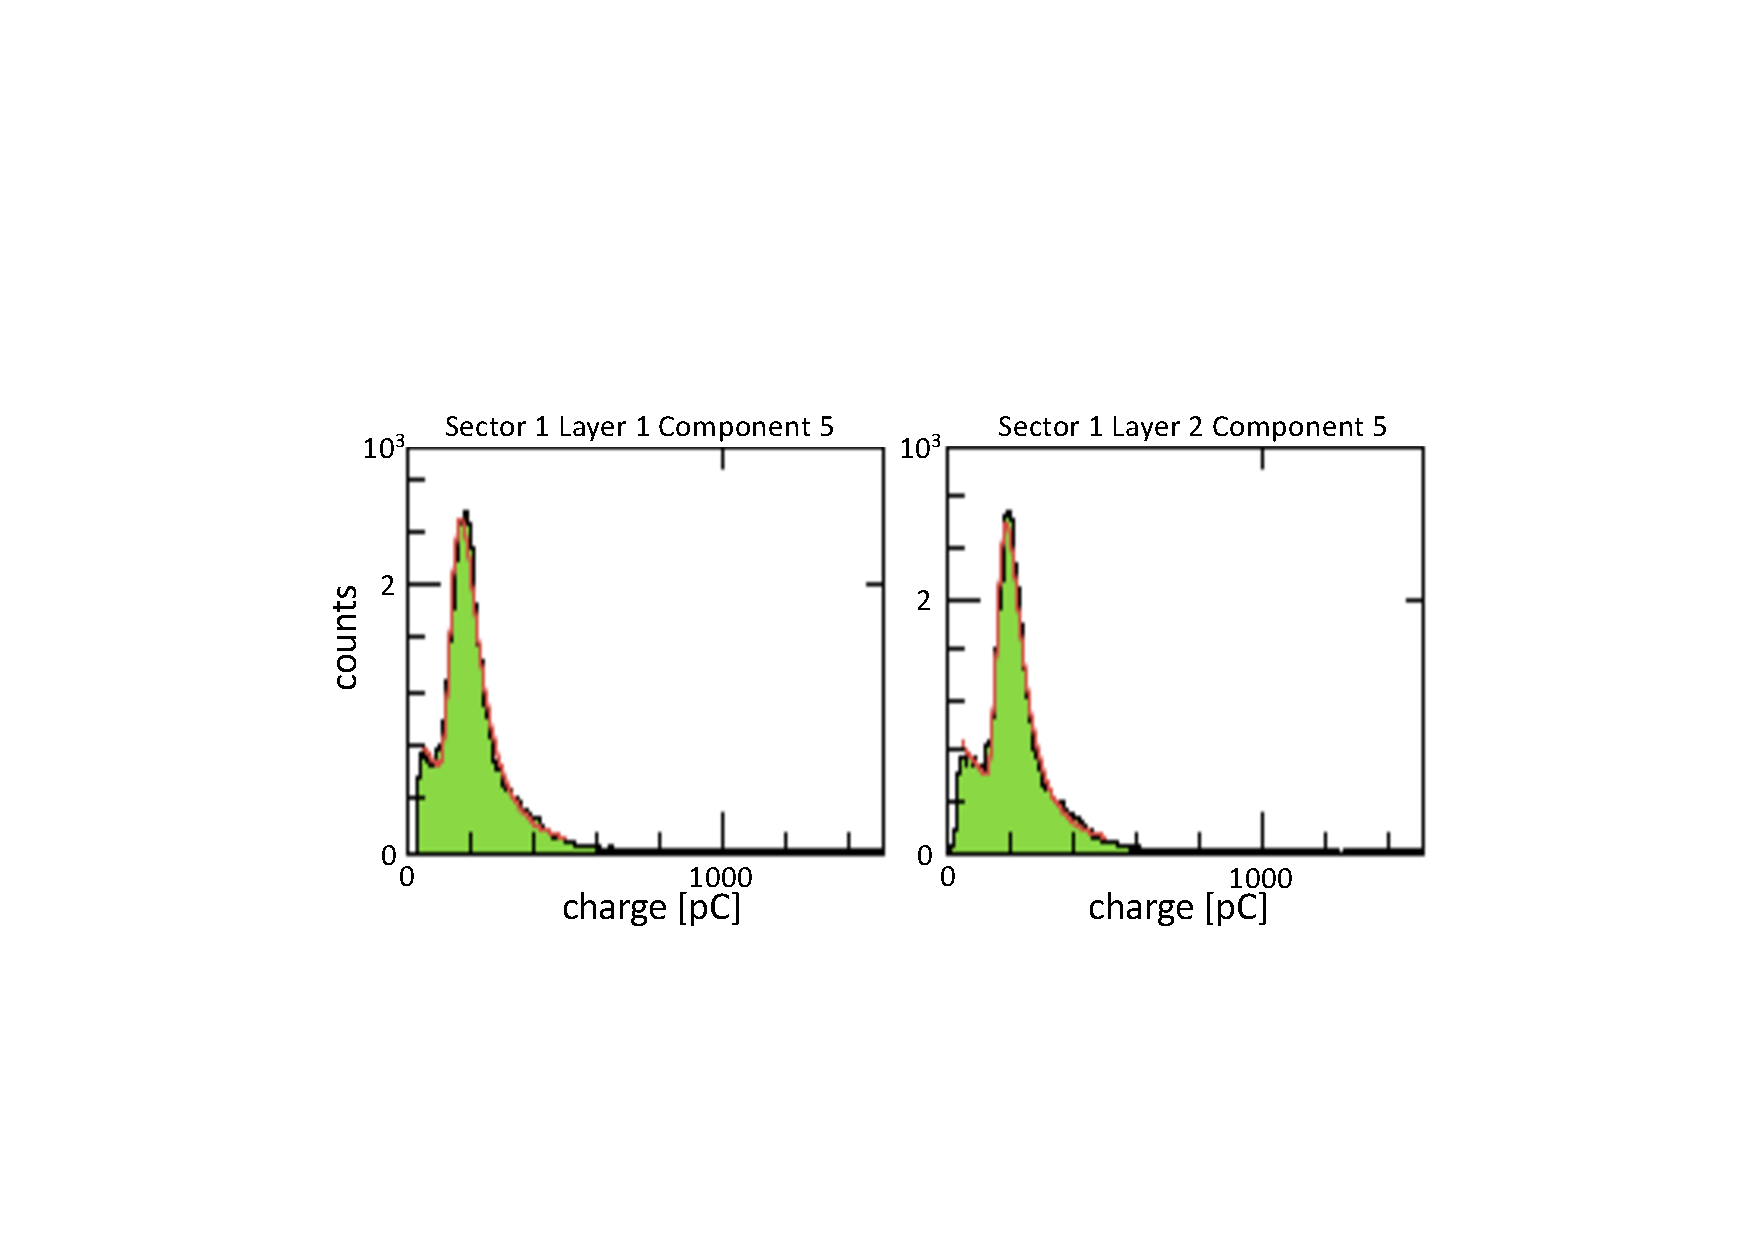
\includegraphics[width=1.0\columnwidth]{fig/fthodo_mips.pdf}
\caption{Signal from two FT-Hodo tiles (thin and thick layer) fitted with a Landau plus an exponential to established
  the charge-to-energy constants.}
\label{fig:fthodo_mips}
\end{figure}

The timing calibrations of both the FT-Cal and FT-Hodo are obtained by studying the time correlation of the signals
detected in the two detectors and the CLAS12 Forward Time-Flight (FTOF) detector~\cite{ftof}. The procedure makes use of events with a
scattered electron in the CLAS12 forward detectors and a second particle detected in the FT. In
such events, the start time $t_0$, i.e. the time of interaction of the beam electron in the target, can be computed
from the electron FTOF time projected back to the event vertex. The start time can then be used as a reference
for the calibration of the FT detectors. 

For the FT-Hodo, the signal time, $t_{hit}$, projected back to the event vertex is compared to the event start time,
$t_0$. The difference between the two gives the time correction needed. Figure~\ref{fig:fthodo_time} shows an
example of the time offset distribution for a thin and a thick tile.

\begin{figure}
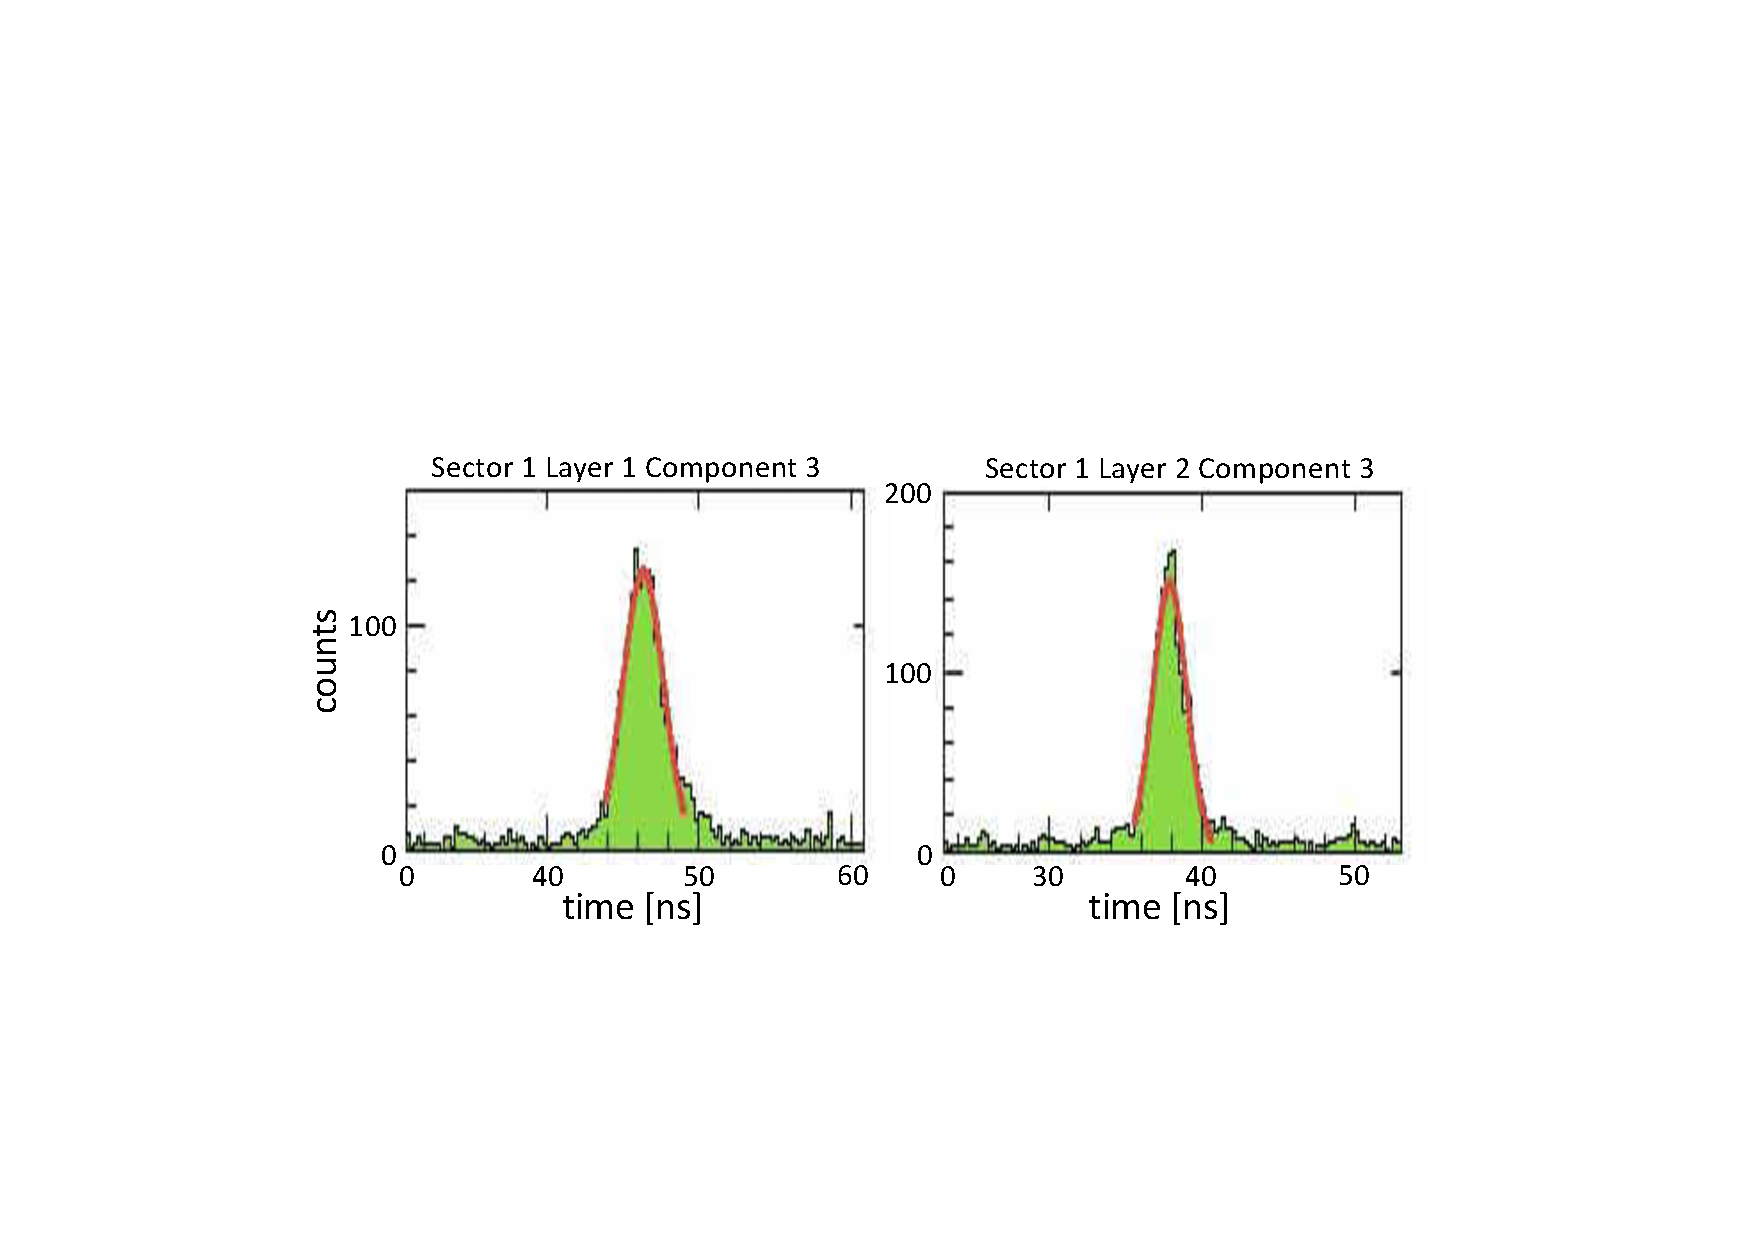
\includegraphics[width=1.0\columnwidth]{fig/fthodo_time.pdf}
\caption{FT-Hodo time correction determined by Gaussian fits on the time difference between the hit time
  projected back to the event vertex and the event start time.}
\label{fig:fthodo_time}
\end{figure}

The same procedure is used for the FT-Cal, for which however all hits with energy greater than 10 MeV are used
with no requirements on the charge of the associated particle. The use of such a low energy threshold is important
to be able to calibrate the crystals that are on the edges of the calorimeter. The measured time is then compared
with the event start time, extracting both an overall offset and a charge-dependent correction, associated with a
time-walk effect. The top-left panel of Fig.~\ref{fig:ftcal_time} shows the time offset as  a function the
signal charge; this histogram profile is fitted to a power law, $a/q^\lambda$, as shown in the top-right panel to
determine the time-walk correction. After applying this correction, the time offset distribution shown in the bottom
plots  of the same figure are fitted to a simple Gaussian function to determine the global offset. The bottom right
plot shows the final distribution with all corrections, showing a clear  coincidence peak at 0 surrounded by the
accidental peaks at multiple of $\pm$4.008~ns  due to the RF beam structure. The time offset constant term is
extracted for each crystal separately, while the time walk constants are fitted for all crystals together since no
significant difference between crystals was found. The resolution achieved with this procedure are reported in Section~\ref{sec:performance}

\begin{figure}
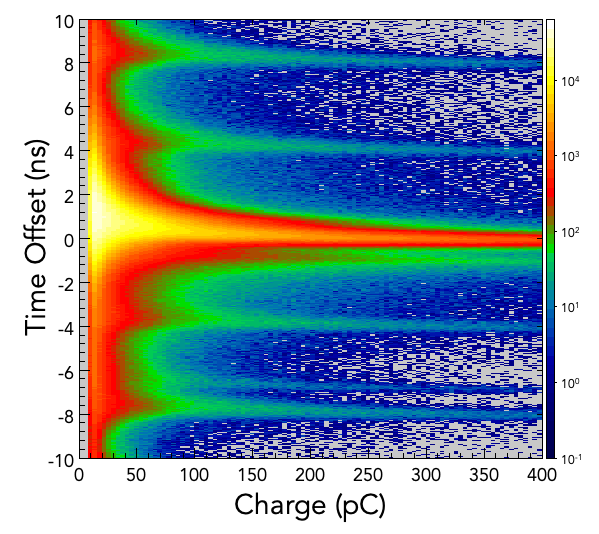
\includegraphics[height=0.42\columnwidth]{fig/ftcal_twbefore.png}
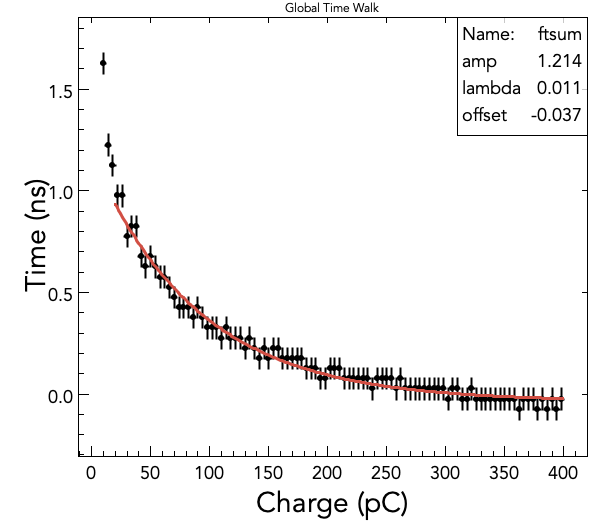
\includegraphics[height=0.42\columnwidth]{fig/ftcal_twfit.png}
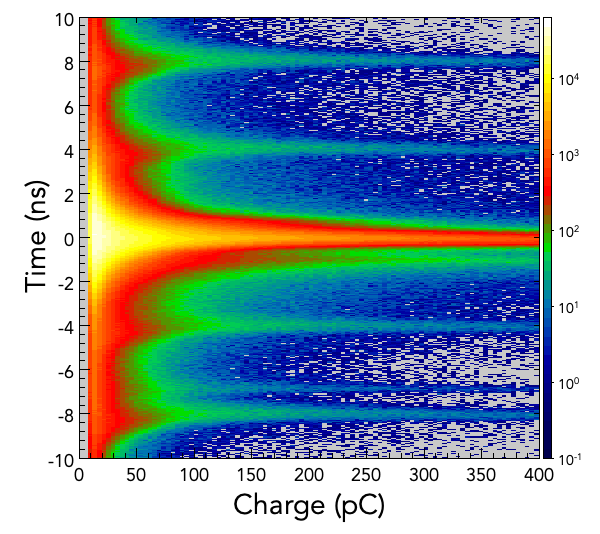
\includegraphics[height=0.42\columnwidth]{fig/ftcal_twafter.png}
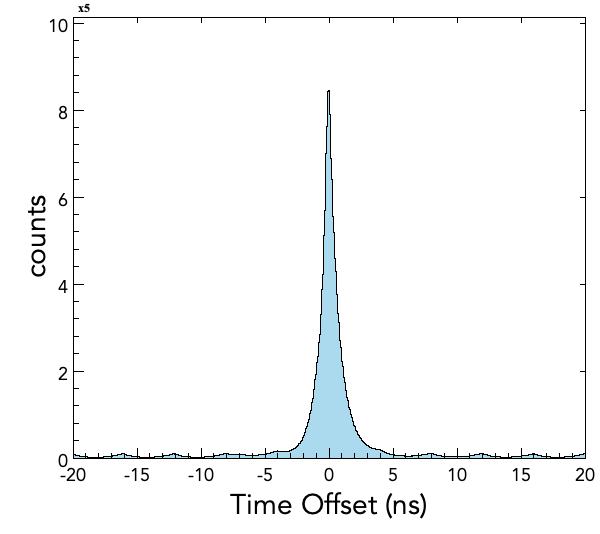
\includegraphics[height=0.42\columnwidth]{fig/ftcal_timefinal.png}
\caption{Top: FT-Cal time offset dependence on the charge (left); the profile of the histogram is fitted to a power
  law, $a/q^\lambda$. Bottom: FT-Cal time offsets after the time walk and the subtraction of the residual constant term.}
\label{fig:ftcal_time}
\end{figure}
